\section{Proof-of-Concept Implementation}
\label{sec:evaluation}

\subsection{Implementation}

In this section, we describe our implementation of the system using the GloMoSim simulation software. Since it is proof-of-concept, we simplify the system. The controller is an application on the same machine running GloMoSim, and so does not require Openflow for communication. We also assume a simple event model wherein we assume that the controller has information about the state of the network and accordingly decides on an action. We add two modules in GloMoSim to receive commands from the controller and to reconfigure or change the MAC protocols of the nodes. We open a socket between the controller and one of the modules in GloMoSim for sending the commands. The other module performs the actual switching of MAC protocols of all the nodes in the simulation. It is also responsible for performing the 4-way handshake between the MAC Manager and the MAC Agents. The abstractions of SDN switch agent, MAC Manager and MAC Agent are merged into these two modules in our implementation. 

\begin{figure}[t]
  \centering
  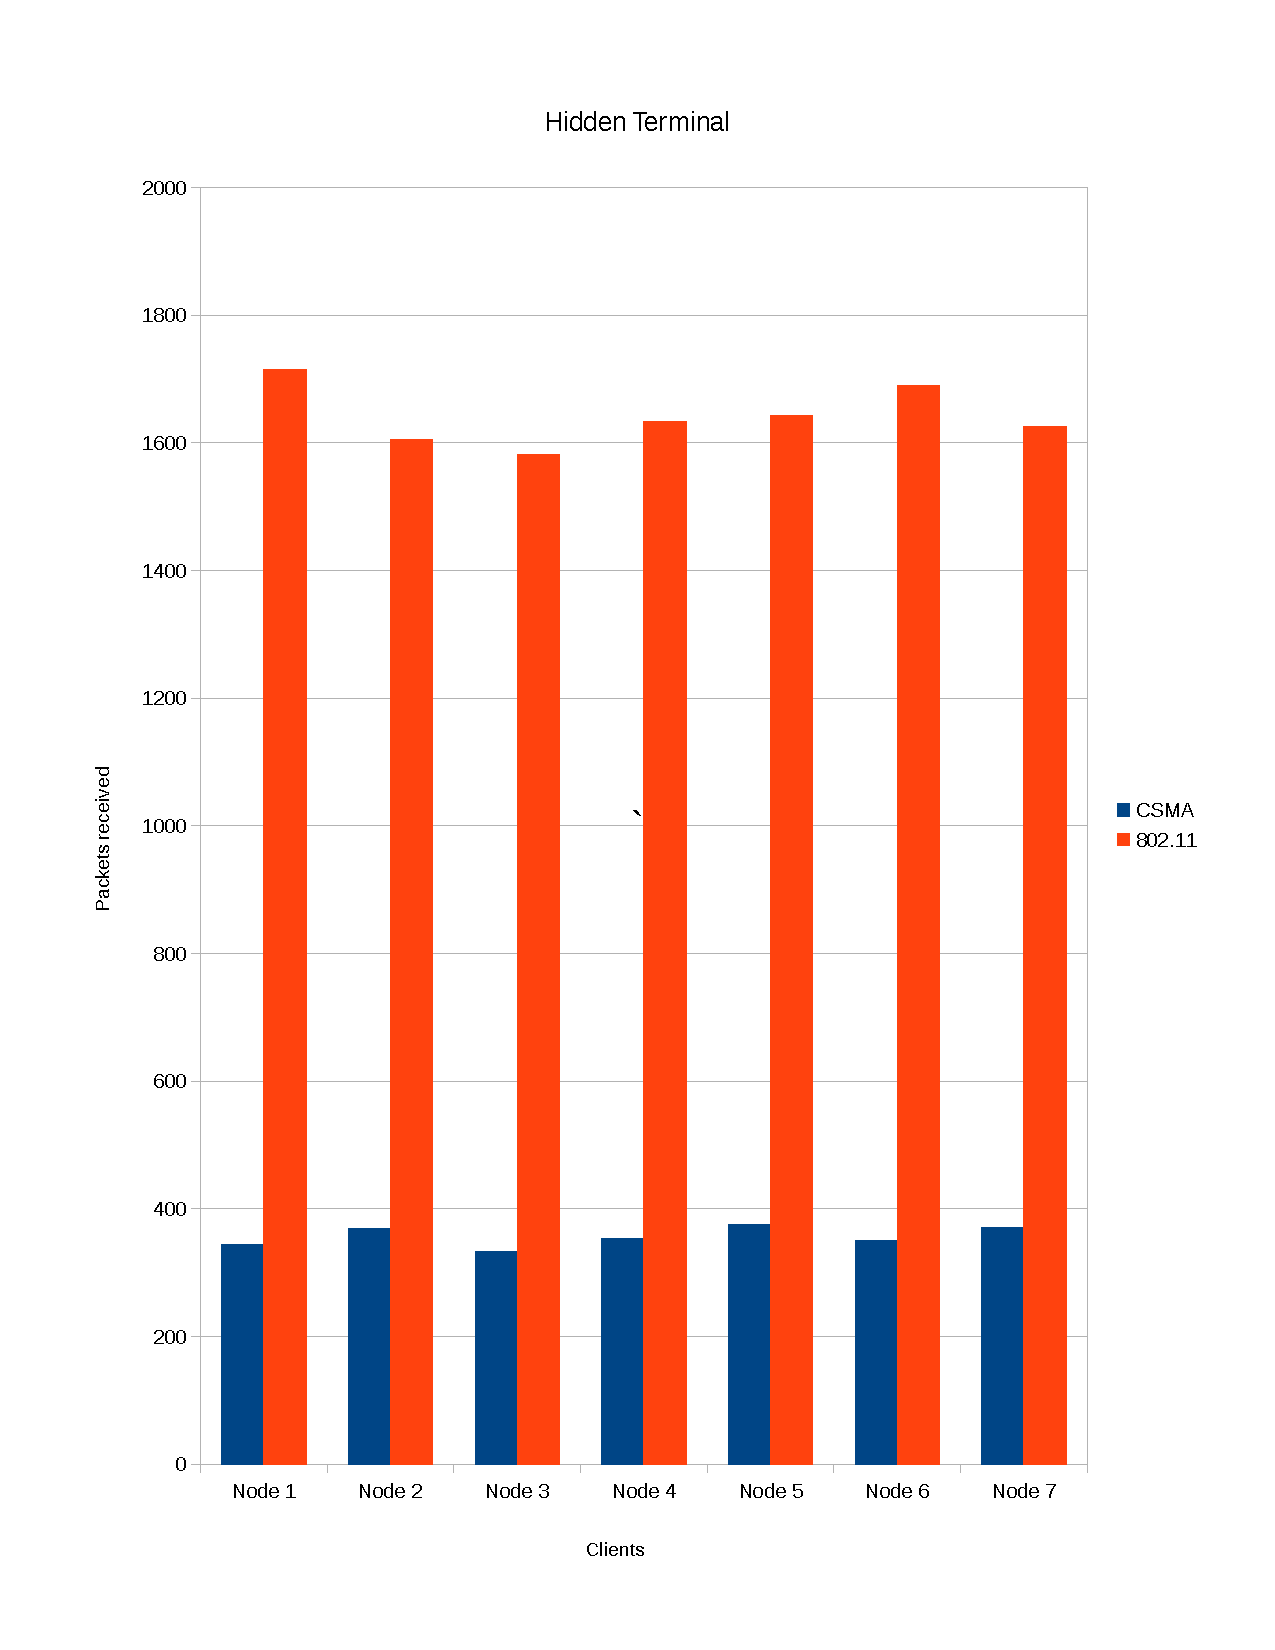
\includegraphics[width=0.35\textwidth, scale=0.35]{figures/hidden_recvPkts.pdf}
  \caption{Change in the number of received packets as the MAC protocol is changed from CSMA to 802.11}
  \label{fig:setup}
\end{figure}

\begin{figure}[t]
  \centering
  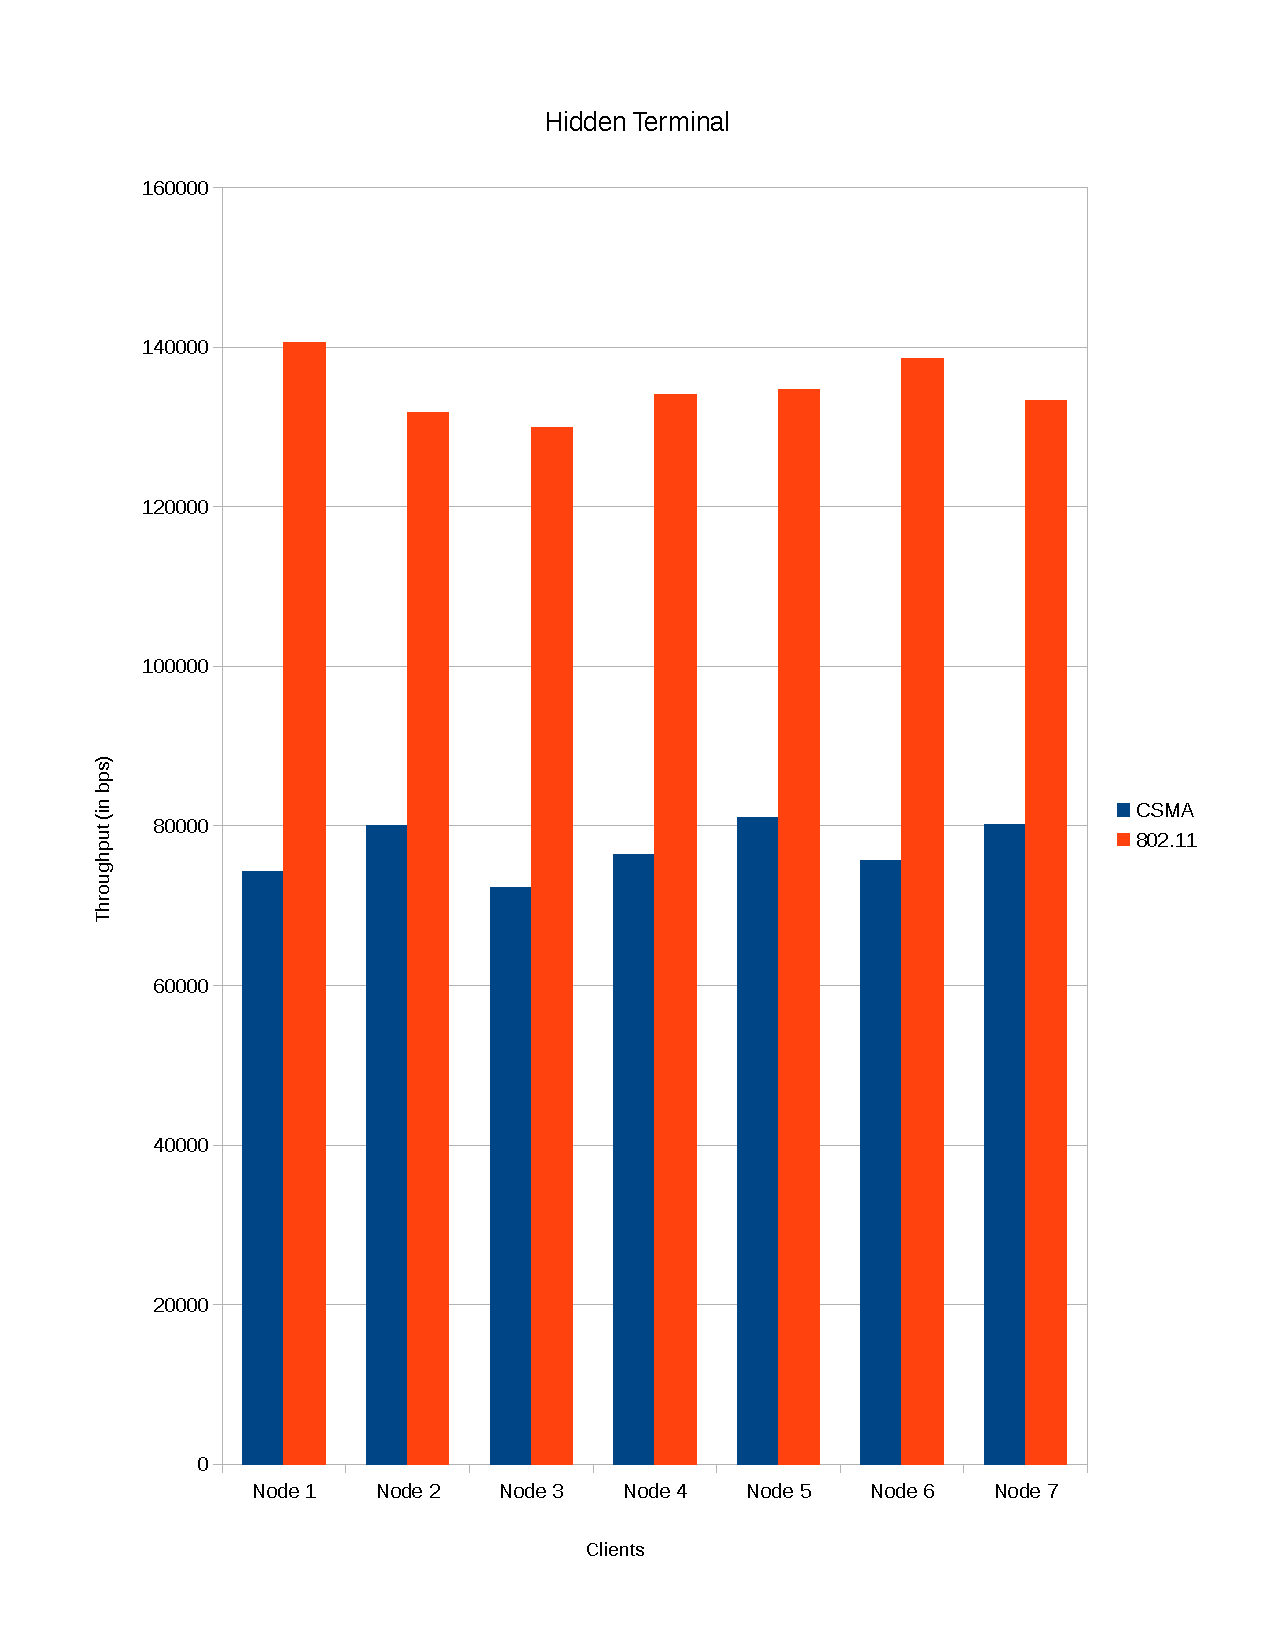
\includegraphics[width=0.35\textwidth, scale=0.35]{figures/hidden_thrput.pdf}
  \caption{Change in throughput of the nodes as the MAC protocol is changed from CSMA to 802.11}
  \label{fig:overhead}
\end{figure}

\begin{figure}[t]
  \centering
  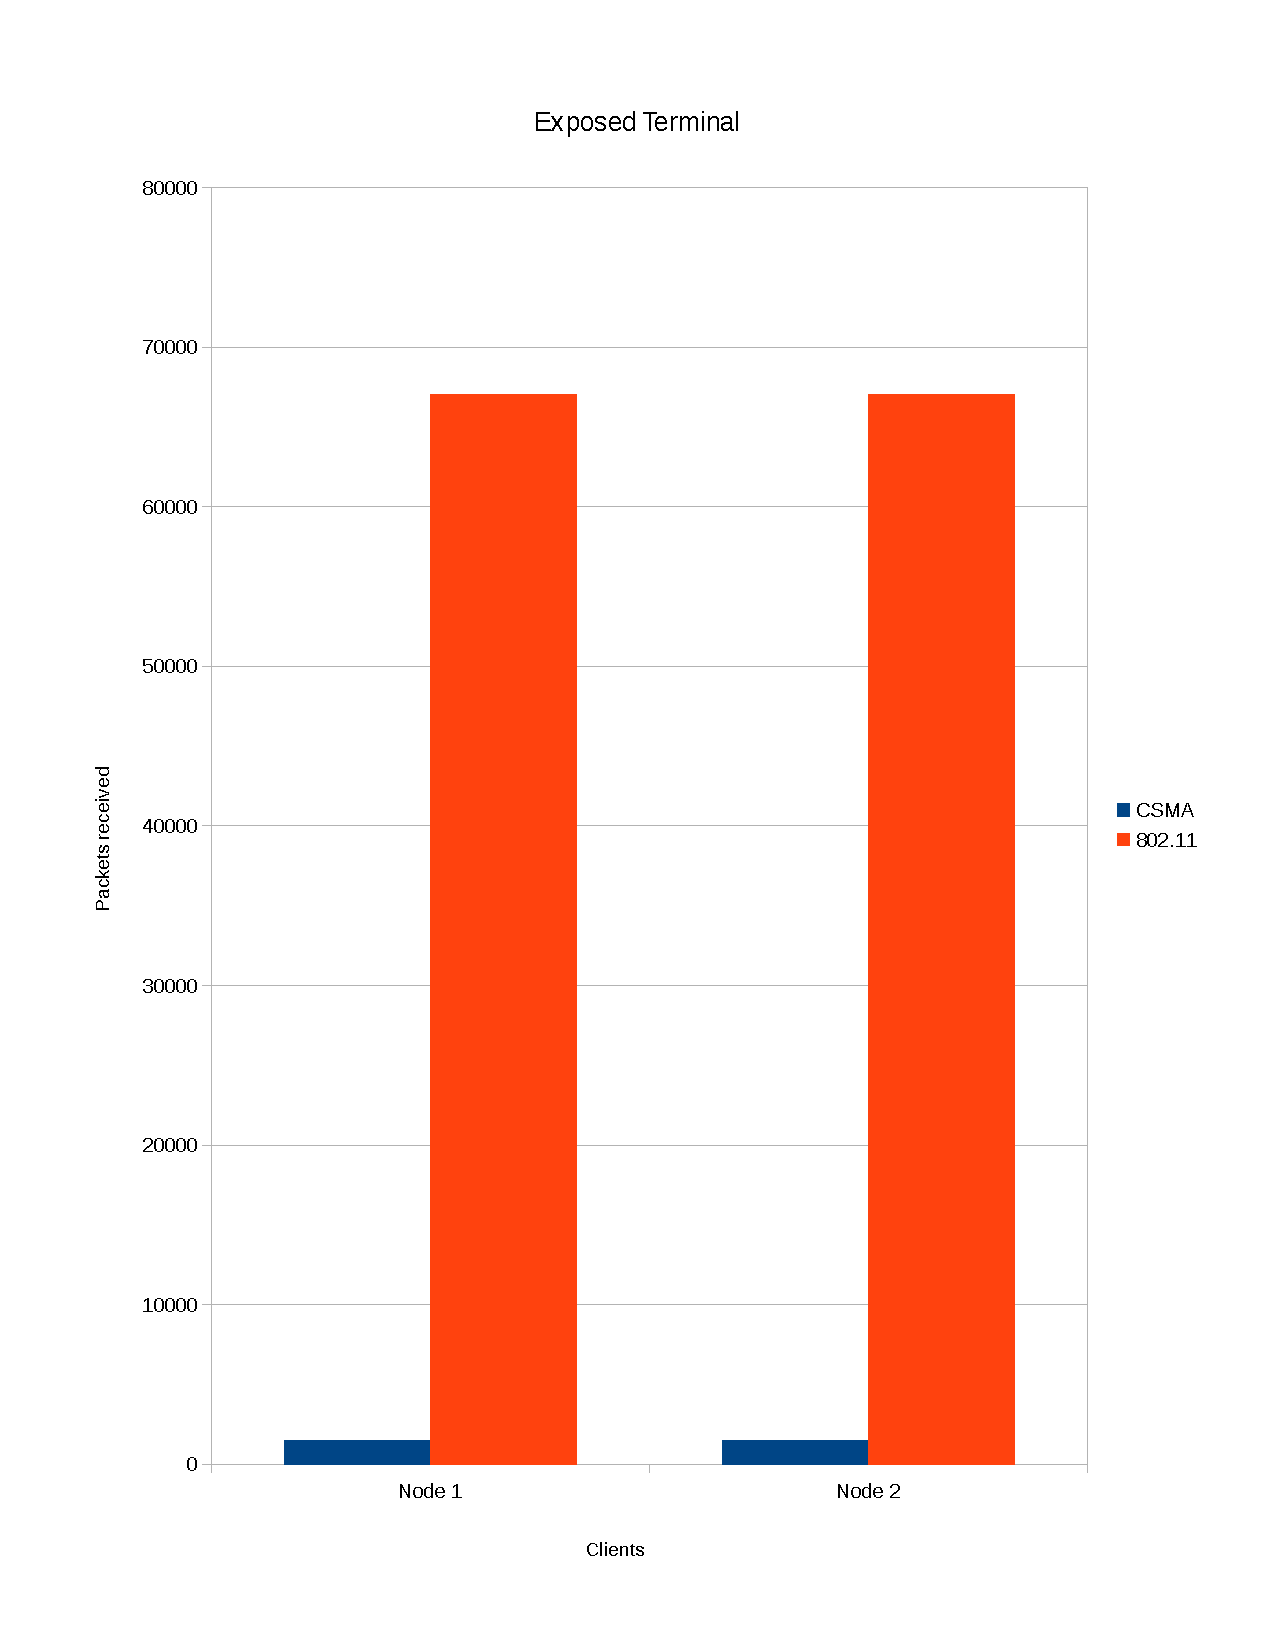
\includegraphics[width=0.35\textwidth, scale=0.35]{figures/exposed_recvPkts.pdf}
  \caption{Change in the number of received packets when the MAC is changed from CSMA to 802.11}
  \label{fig:setup}
\end{figure}

\begin{figure}[t]
  \centering
  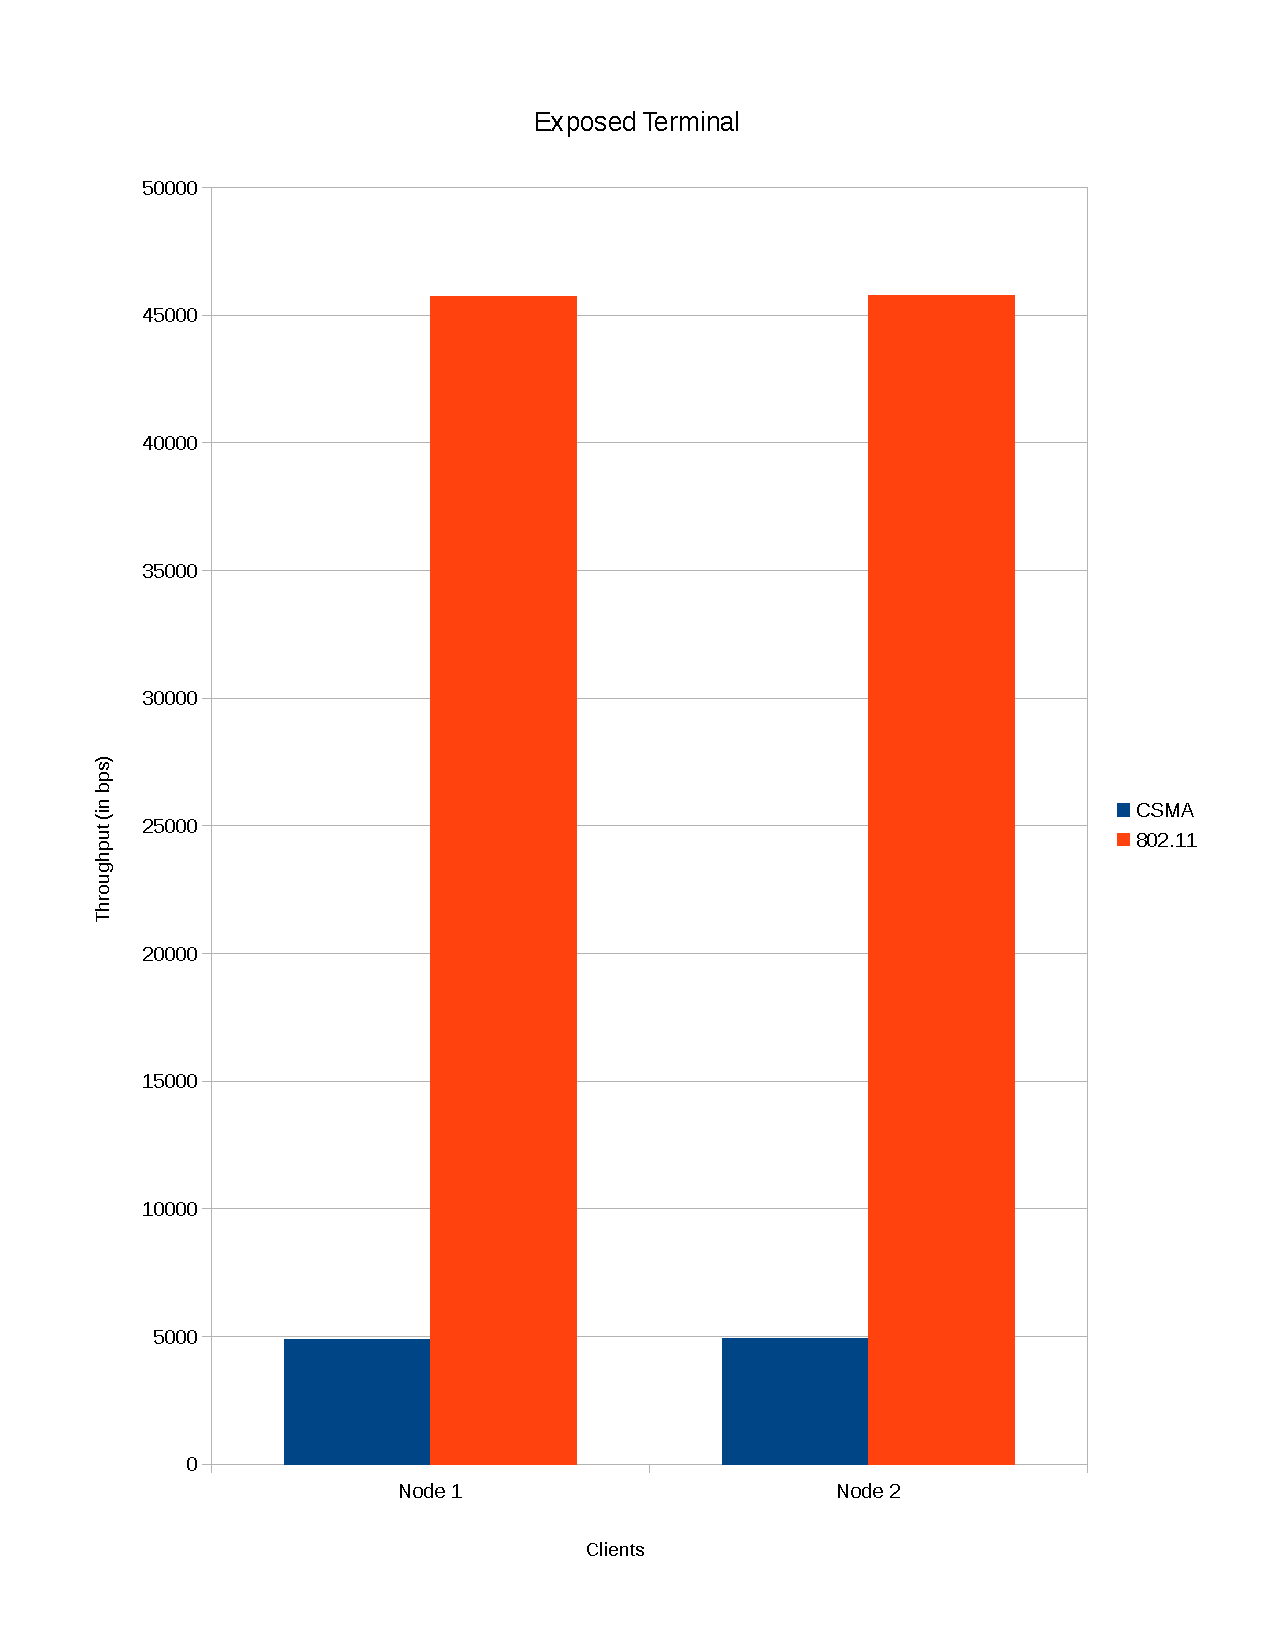
\includegraphics[width=0.35\textwidth, scale=0.35]{figures/exposed_thrput.pdf}
  \caption{Change in the throughput when the MAC protocol is changed from CSMA to 802.11}
  \label{fig:overhead}
\end{figure}

\subsection{Sample Use Cases}

\subsubsection{Hidden Terminal}
The Hidden terminal problem occurs in wireless networks when a node is visible from a particular destination node, but is not visible from other nodes that are communicating with the destination node. Since the transmitting nodes are out of range of one another, CSMA cannot detect a transmission and collisions occur as a result. IEEE 802.11 solves this problem with the help of the RTS/CTS mechanism. Since all trasmitting nodes are within communication range of the destination, they can hear the CTS destined to a particular transmitter. This ensures that only one transmitter communicates with the node. 

We start the simulation with all nodes running CSMA as the MAC protocol. The test controller then issues the \emph{SWITCH-MAC} command with the appropriate MAC protocol (WIFI-PROTO) and forwards the request to all the nodes in the simulation. On each node, we first wait for the in-flight packets to be serviced and the state of the radio to become idle, and then initialize the MAC protocol to 802.11. Waiting for the radios to become idle is an approximation of the 4-way handshake described earlier. We also ensure that the simulation statistics of the nodes under both the original and the changed MAC protocols are saved in glomo.stat. As it is evident from the plots, 802.11 out performs CSMA both in throughput and the number of packets successfully received.

\subsubsection{Exposed Terminal}
The Exposed Terminal problem occurs in wireless networks when a node is not allowed to send packets to other nodes because of the presence of a transmitting node within its radio range, even though the receivers of the two nodes are out of range of each other. In CSMA, a node that wants to send packets performs carrier sense and after sensing the neighbours transmission, decides not to transmit as it would result in interfernce. IEEE 802.11, on the other hand, solves this problem with the help of the RTS/CTS mechansim. A node can identify itself as an exposed node if it hears an RTS from a neighbouringnode, but does not hear a corresponding CTS. It can then transmit to its intended receivers. 
Similar to the \emph{Hidden terminal} use case, we start the simulation with all the nodes running CSMA and then, the test controller issues the \emph{SWTICH-MAC} command with the appropriate MAC protocol (WIFI-PROTO) and forwards the request to all the nodes in the simulation. On each node, we wait for the in-flight packets to be serviced and the state of the radio to become idle, and then initialize the MAC protocol to 802.11, which is the approximation for the 4-way handshake. We also ensure that the simulation statistics of the nodes under both MAC protocols are saved in glomo.stat. As it is evident from the plots, 802.11 out performs CSMA both in throughput and the number of packets successfully received.  
